
% !TEX TS-program = pdflatex
% !TEX encoding = UTF-8 Unicode


%%%%%%%%%%%%%%%%%%%%%%%%%%%%%%%%%%%%%%%%%%%%%%%%%%%%%%%%%%%%%%%%%%%%%%
%%%%%%%%%%%%%%%%%%%%%%%%%%%%%%	HEADER %%%%%%%%%%%%%%%%%%%%%%%%%%%%%%%%%%%%
\documentclass[12pt]{article} 
\usepackage{amsmath, amsthm, amssymb} % AMS Math Package
\usepackage{graphicx} % Allows for eps images
\usepackage{multicol} % Allows for multiple columns
\usepackage{framed,color}
\usepackage{fancybox}
\usepackage{float}
\usepackage{caption,subcaption}
\usepackage{mathtools}
\usepackage{float}
\usepackage{textcomp}

\usepackage{geometry}
\geometry{
top=0.5in,
inner=0.5in,
outer=0.5in,
bottom=0.5in,
headheight=1ex,
headsep=3ex
}


 % Sets margins and page size
\pagestyle{empty} % Removes page numbers
\makeatletter % Need for anything that contains an @ command 
\renewcommand{\maketitle} % Redefine maketitle to conserve space
{ \begingroup \vskip 10pt \begin{center} \large {\bf \@title}
	\vskip 10pt \large \@author \hskip 20pt \@date \end{center}
  \vskip 10pt \endgroup \setcounter{footnote}{0} }
\makeatother % End of region containing @ commands
\renewcommand{\labelenumi}{(\alph{enumi})} % Use letters for enumerate
% \DeclareMathOperator{\Sample}{Sample}
\let\vaccent=\v % rename builtin command \v{} to \vaccent{}
\renewcommand{\v}[1]{\ensuremath{\mathbf{#1}}} % for vectors
\newcommand{\gv}[1]{\ensuremath{\mbox{\boldmath$ #1 $}}} 
% for vectors of Greek letters
\newcommand{\uv}[1]{\ensuremath{\mathbf{\hat{#1}}}} % for unit vector
\newcommand{\abs}[1]{\left| #1 \right|} % for absolute value
\newcommand{\avg}[1]{\left< #1 \right>} % for average
\let\underdot=\d % rename builtin command \d{} to \underdot{}
\renewcommand{\d}[2]{\frac{d #1}{d #2}} % for derivatives
\newcommand{\dd}[2]{\frac{d^2 #1}{d #2^2}} % for double derivatives
\newcommand{\pd}[2]{\frac{\partial #1}{\partial #2}} 
% for partial derivatives
\newcommand{\pdd}[2]{\frac{\partial^2 #1}{\partial #2^2}} 
% for double partial derivatives
\newcommand{\pdc}[3]{\left( \frac{\partial #1}{\partial #2}
 \right)_{#3}} % for thermodynamic partial derivatives
\newcommand{\ket}[1]{\left| #1 \right>} % for Dirac bras
\newcommand{\bra}[1]{\left< #1 \right|} % for Dirac kets
\newcommand{\braket}[2]{\left< #1 \vphantom{#2} \right|
 \left. #2 \vphantom{#1} \right>} % for Dirac brackets
\newcommand{\matrixel}[3]{\left< #1 \vphantom{#2#3} \right|
 #2 \left| #3 \vphantom{#1#2} \right>} % for Dirac matrix elements
\newcommand{\grad}[1]{\gv{\nabla} #1} % for gradient
\let\divsymb=\div % rename builtin command \div to \divsymb
\renewcommand{\div}[1]{\gv{\nabla} \cdot #1} % for divergence
\newcommand{\curl}[1]{\gv{\nabla} \times #1} % for curl
\let\baraccent=\= % rename builtin command \= to \baraccent
\renewcommand{\=}[1]{\stackrel{#1}{=}} % for putting numbers above =
\newtheorem{prop}{Proposition}
\newtheorem{thm}{Theorem}[section]
\newtheorem{lem}[thm]{Lemma}
\theoremstyle{definition}
\newtheorem{dfn}{Definition}
\theoremstyle{remark}
\newtheorem*{rmk}{Remark}

\usepackage[utf8]{inputenc} % set input encoding (not needed with XeLaTeX)
\usepackage{tikz} %for making pretty figures
\usepackage[tikz]{bclogo}
\usepackage{tikz-3dplot}
\usetikzlibrary{calc}

%%% HEADERS & FOOTERS
\usepackage{fancyhdr}
\setlength{\headheight}{15pt}
\pagestyle{fancyplain}
\usepackage{lastpage}
\usepackage{siunitx}
\pagenumbering{arabic}

\lhead{Kyle Hoke}
\chead{PHYS 243A, Homework 4\rightmark}
\rhead{Page \thepage\ / \pageref{LastPage}}
\renewcommand{\headrulewidth}{0.4pt}
\fancyfoot[C]{}

%%% section* TITLE APPEARANCE
\usepackage{sectsty}
\allsectionsfont{\sffamily\mdseries\upshape} % (See the fntguide.pdf for font help)

%%% User Defined Commands %%%%
\newcommand{\f}[1]{f_{#1}(x)}
\newcommand{\axis}{
		\draw[->,thick](0,0) -- (0,5);
		\node[above] at (0,5) {$x$};
		\draw[->,thick](0,0) -- (5,0);
		\node[right] at(5,0){$y$};
		}

%%%%%%%%%%%%%%%%%%%%%%%%%%%%%%%%%%%%%%%%%%%%%%%%%%%%%%%%%%%%%%%%%%%%%%%%%%%%%%%
%%%%%%%%%%%%%%%%%%%%%%%%%%%%%%%%%%%%%% END OF HEADER %%%%%%%%%%%%%%%%%%%%%%%%%%%%%%%%%
%%%%%%%%%%%%%%%%%%%%%%%%%%%%%%%%%%%%%%%%%%%%%%%%%%%%%%%%%%%%%%%%%%%%%%%%%%%%%%%





%%% BEGIN DOCUMENT %%%%%%%%%%%%%%%%%%%%%%%%%%%%%%%%%%%%%%%%%%%%%%%%%%%%%%%%%%%%%%%%%%%
\title{\LARGE PHYS 243A Homework 4}
\author{Kyle Hoke}
%\date{} % Activate to display a given date or no date (if empty),
         % otherwise the current date is printed 

\begin{document}
\maketitle
\thispagestyle{empty}





%%%%%%%%%%%%%%%%%%%%%%%%%%%%%%%%%%%%%%%%%%%%%%%%%%%%%%%%%%%%%%%%%%%%%%%%%%%%%%%%%%%%
%%%%%%%%%%%%%%% PROBLEM 1 %%%%%%%%%%%%%%%%%%%%%
%%%%%%%%%%%%%%%%%%%%%%%%%%%%%%%%%%%%%%%%%%%%%%%%%%%%%%%%%%%%%%%%%%%%%%%%%%%%%%%%%%%%

\section*{4.5}
\subsection*{a}

\begin{figure}[H]
\centering
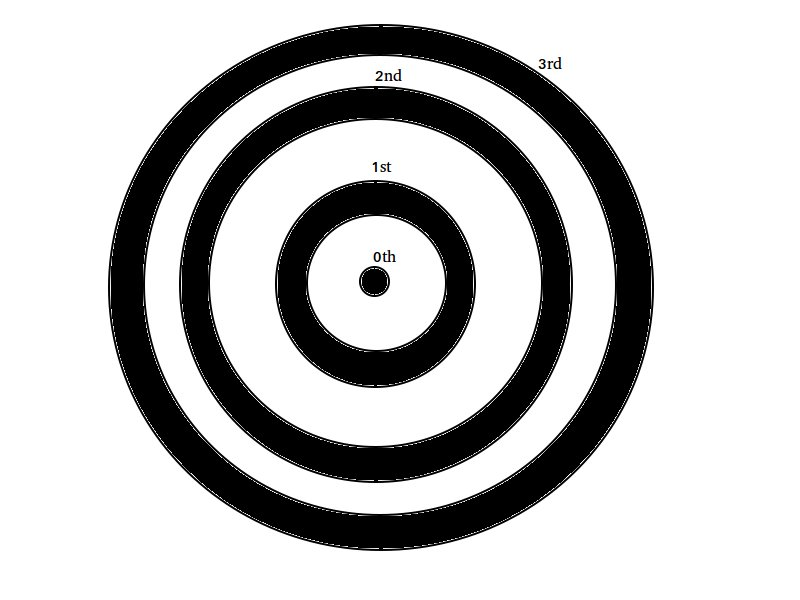
\includegraphics[scale=0.5]{./images/4-5a.jpg}
\caption{Basic diffraction pattern of C 1s excitation with the order of the dirraction ring written in on the image.}
\label{4-5a}
\end{figure}


\subsection*{b}
\begin{align*}
KE &= h\nu - E_b \\[3mm]
	&= 1486.6 - 284.2\\[3mm]
	&= 1204.4 \,\,\text{eV}
\end{align*}

Using this kinetic energy we can calculate the wavelength of the diffracted electron via,

\begin{align*}
\lambda &= \dfrac{h}{\sqrt{2mKE}}\\[3mm]
	&= 0.35\,\,\AA
\end{align*}

This implies a wavenumber of \(|k| = 18\,\,\AA^{-1}\). We are given that $r_{oxy}=1.1\,\,\AA$ so we can conclude 
that the number of partial-wave scattering phase shifts to be calculated is about
\begin{align*}
l &= |k|\cdot r_{oxy}\\[3mm]
	&= 19.8 \implies 20 \,\,\text{partial waves}
\end{align*}

\subsection*{c}
First order, n=1, with $\theta_{Co} = 40^\circ$ for normal first-order scattering angle. We use the following equation,
\begin{align*}
2\pi &= |k|\cdot r_{Co}\cdot \left(1-\cos\theta_{Co}\right) +\Psi_0(\theta)\\[3mm]
\Psi_0(\theta) &= 2\pi - (18\,\AA)\cdot(1.18\,\AA)\cdot(1-\cos(40^\circ))\\[3mm]
	&= 1.31 \implies \theta \approx 78^\circ
\end{align*}

The scattering phase shift is about 78 degrees.

\subsection*{d}
Parameters used:
\begin{align*}
&\text{atom}\quad O\quad 0\quad 0\quad 1.83 &\text{electron energy: } 1000\,\,\text{eV}\\[2mm]
&\text{atom}\quad C\quad 0\quad 0\quad 3.01 &\text{incidence angle: } 89^\circ\\[2mm]
&\text{atom}\quad Ni\quad 0\quad 0\quad 0   &\text{Debye Temp: } 450\,\,\text{K}\\[2mm]
&\text{emitter}\quad O\quad 0\quad 0\quad 0 &V_0= 14\,\,\text{eV}\\[2mm]
&\text{end} 								&\rho= 8.9\,\,\text{g/cm$^3$}
\end{align*}

\begin{figure}[H]
\centering
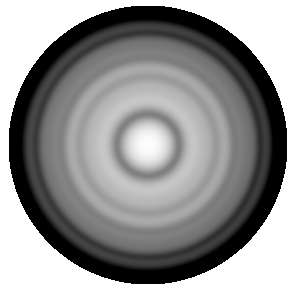
\includegraphics[scale=0.5]{./images/4-5d.png}
\caption{1st order}
\label{4-5d}
\end{figure}

\begin{figure}[H]
\centering
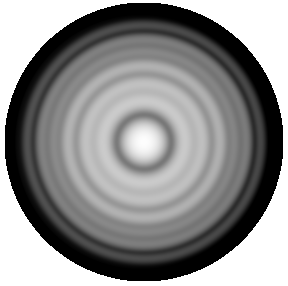
\includegraphics[scale=0.5]{./images/4-5d2.png}
\caption{6th order}
\label{4-5d2}
\end{figure}

\subsection*{e}
Parameters used:
\begin{align*}
&\text{atom}\quad O\quad 0\quad 0\quad 1.83 &\text{electron energy: } 100\,\,\text{eV}\\[2mm]
&\text{atom}\quad C\quad 0\quad 0\quad 3.01 &\text{incidence angle: } 89^\circ\\[2mm]
&\text{atom}\quad Ni\quad 0\quad 0\quad 0   &\text{Debye Temp: } 450\,\,\text{K}\\[2mm]
&\text{emitter}\quad O\quad 0\quad 0\quad 0 &V_0= 14\,\,\text{eV}\\[2mm]
&\text{end} 								&\rho= 8.9\,\,\text{g/cm$^3$}
\end{align*}

\begin{figure}[H]
\centering
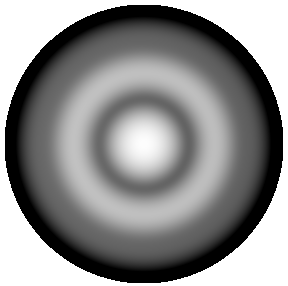
\includegraphics[scale=0.5]{./images/4-5e.png}
\caption{1st order}
\label{4-5e}
\end{figure}
%%%%%%%%%%%%%%%%%%%%%%%%%%%%%%%%%%%%%%%%%%%%%%%%%%%%%%%%%%%%%%%%%%%%%%%%%%%%%%%%%%%%
%%%%%%%%%%%%%%% PROBLEM 2 %%%%%%%%%%%%%%%%%%%%%
%%%%%%%%%%%%%%%%%%%%%%%%%%%%%%%%%%%%%%%%%%%%%%%%%%%%%%%%%%%%%%%%%%%%%%%%%%%%%%%%%%%%
\newpage
\section*{4.7a}
The grating equation is 
\[
\sin\theta_{inc} + \sin\theta_{refl} = \dfrac{m\lambda}{d}
\]
We solve for $\lambda$, then take the derivative of lambda w.r.t. the reflected angle.
\[
\lambda = \dfrac{d}{m}\left(\sin\theta_{inc} + \sin\theta_{refl}\right)
\]
\[
\d{\lambda}{\theta_{refl}} = \dfrac{d}{m}\cos\theta_{refl}
\]

Thus the dispersion of the grating is,

\[
\d{\theta_{refl}}{\lambda} = \dfrac{m}{d\cos\theta_{refl}}
\]

To maximize this values we want to minimize $d$. The reflected angle is not something we can control, but we 
can look for reflections that have values close to 90 degrees.

%%%%%%%%%%%%%%%%%%%%%%%%%%%%%%%%%%%%%%%%%%%%%%%%%%%%%%%%%%%%%%%%%%%%%%%%%%%%%%%%%%%%
%%%%%%%%%%%%%%% PROBLEM 3 %%%%%%%%%%%%%%%%%%%%%
%%%%%%%%%%%%%%%%%%%%%%%%%%%%%%%%%%%%%%%%%%%%%%%%%%%%%%%%%%%%%%%%%%%%%%%%%%%%%%%%%%%%
\newpage
\section*{5.1}
\subsection*{a}
\begin{figure}[H]
\centering
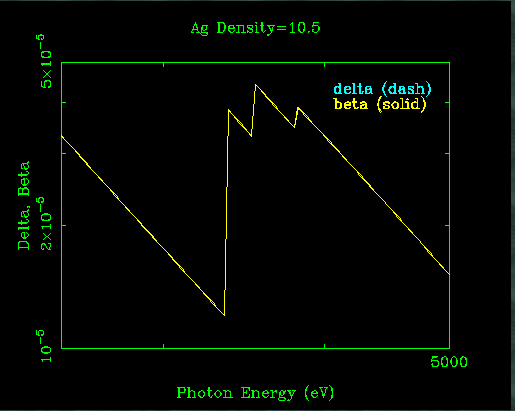
\includegraphics[scale=0.7]{./images/5-1a.png}
\caption{Index of refraction for Ag}
\label{5-1a}
\end{figure}

The two small adsorption edges after the main edge are evidence of spin orbit splitting. The edges are L1, L2 and L3.

\subsection*{b}
The critical angle for total external reflection can be calculated from the real part of the refractive index via,
\[
\theta_C = \sqrt{2\delta}
\]

Using a tables of values generated from the above plot we get,

\begin{align*}
\theta_C &= \sqrt{2 \cdot 0.00011}\\[3mm]
	&\approx 0.02 \,\,\text{rad}\\[3mm]
	&= 1.1^\circ
\end{align*}

\begin{figure}[H]
\centering
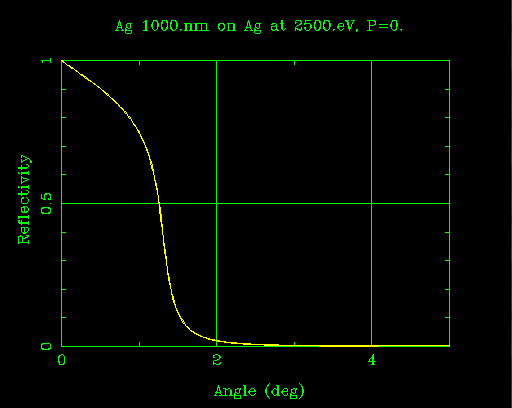
\includegraphics[scale=0.7]{./images/5-1b.png}
\caption{Reflectivity for Ag}
\label{5-1b}
\end{figure}

The critical angle is at the inflection point in the above figure; this value agrees fairly well with the value of 1.1$^\circ$.

\subsection*{c}
\begin{figure}[H]
\centering
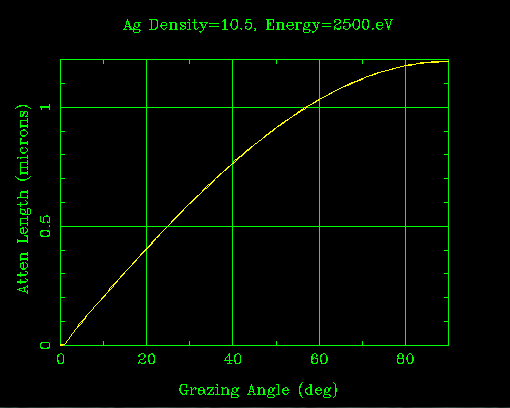
\includegraphics[scale=0.7]{./images/5-1c.png}
\caption{Attenuation length for Ag}
\label{5-1c}
\end{figure}

\begin{figure}[H]
\centering
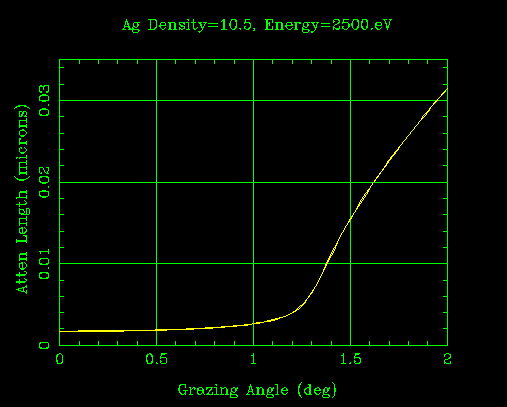
\includegraphics[scale=0.7]{./images/5-1c2.png}
\caption{Attenuation length for Ag below the critical angle.}
\label{5-1c2}
\end{figure}

After replotting the data as a function of Sin($\theta$) we determine that the behavior of the attenuation length is similar to electron escape depth in the overlayer up to about 15-20 nanometers
%%%%%%%%%%%%%%%%%%%%%%%%%%%%%%%%%%%%%%%%%%%%%%%%%%%%%%%%%%%%%%%%%%%%%%%%%%%%%%%%%%%%
%%%%%%%%%%%%%%% PROBLEM 4 %%%%%%%%%%%%%%%%%%%%%
%%%%%%%%%%%%%%%%%%%%%%%%%%%%%%%%%%%%%%%%%%%%%%%%%%%%%%%%%%%%%%%%%%%%%%%%%%%%%%%%%%%%
\newpage
\section*{5.2}
\subsection*{a}

\begin{figure}[H]
\centering
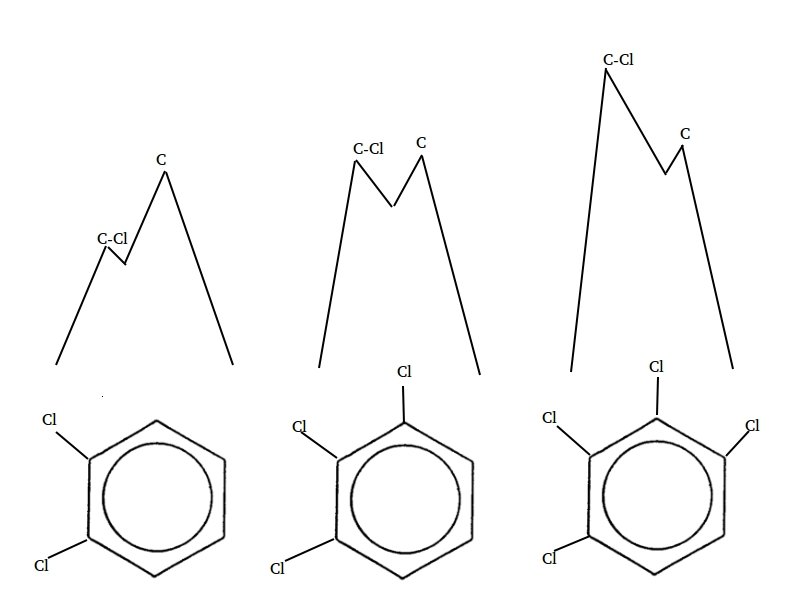
\includegraphics[scale=0.6]{./images/5-2a.jpg}
\label{5-2a}
\end{figure}

Predications are consistent as the ration in intensities are related to the ratio of C-Cl and carbons without a Cl attached.

\subsection*{b}
\[
E_b(k) = E_b(k, q_A) + V
\]
\[
\text{compound} = \text{free ion of charge $q_a$} + \text{Potential due to all other atoms}
\]
284.2 eV is the 1s binding energy for carbon (CXRO data tables). 23.3 eV is the potential due to being bond to a Cl atom.

\subsection*{c}
Coloumb integral = 23.3 eV

\subsection*{d}
284.9 eV is the 1s binding energy of a FREE carbon atom.

%%%%%%%%%%%%%%%%%%%%%%%%%%%%%%%%%%%%%%%%%%%%%%%%%%%%%%%%%%%%%%%%%%%%%%%%%%%%%%%%%%%%
%%%%%%%%%%%%%%% PROBLEM 5 %%%%%%%%%%%%%%%%%%%%%
%%%%%%%%%%%%%%%%%%%%%%%%%%%%%%%%%%%%%%%%%%%%%%%%%%%%%%%%%%%%%%%%%%%%%%%%%%%%%%%%%%%%
\newpage
\section*{5.3}

\subsection*{a}
Ground state electronic configuration:
\[
\text{1s electrons = } 1s_o^2 1s_N^2 3\sigma^2 4{\sigma^*}^2 5\sigma^2 1\pi^4 2{\pi^*}^1
\]

\subsection*{b}
\begin{align*}
K_{O_{1s}, 2\pi} \to O1s\\[2mm]
K_{N_{1s}, 2\pi} \to N1s
\end{align*}

\subsection*{c}
$N_{1s,2\pi}$ is larger which means $K_{N_{1s}, 2\pi}$ is larger; this is due to the larger radius of the N atom compared to oxygen. This larger radius means a larger sphere of influence, and thus a larger repulsive potential.

\subsection*{d}

%%%%%%%%%%%%%%%%%%%%%%%%%%%%%%%%%%%%%%%%%%%%%%%%%%%%%%%%%%%%%%%%%%%%%%%%%%%%%%%%%%%%
%%%%%%%%%%%%%%% PROBLEM 6 %%%%%%%%%%%%%%%%%%%%%
%%%%%%%%%%%%%%%%%%%%%%%%%%%%%%%%%%%%%%%%%%%%%%%%%%%%%%%%%%%%%%%%%%%%%%%%%%%%%%%%%%%%
\newpage
\section*{5.4}

\subsection*{a}
All of the 4p bands look parabolic, which is indicative of free electron like behavior. The flatter bands at the bottom are probably the 4d bands, which are completely full in Ga.

\subsection*{b}
These are most likely the d-electrons which are at a much higher binding energy than they would be in a transition metal because the d-orbitals are full.

\subsection*{c}
\begin{figure}[H]
\centering
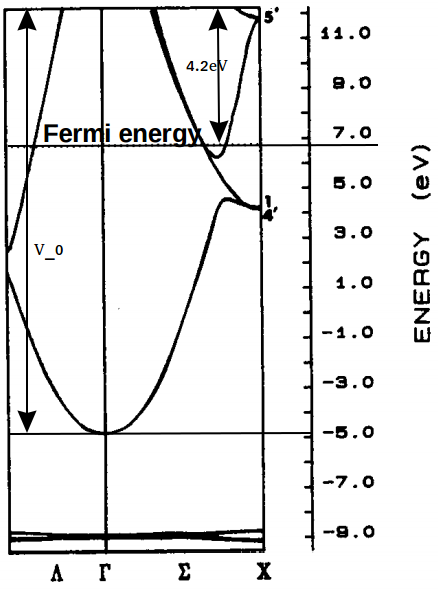
\includegraphics[scale=0.6]{./images/5-4c.png}
\label{5-4c}
\end{figure}

The work function of Ga is 4.2eV. The inner potential for this plot is roughly,
\begin{align*}
V_0 &= -(-5eV) + 6.9eV + 4.2eV\\[2mm]
	&= 16.1 \,\, \text{eV}
\end{align*}

%%%%%%%%%%%%%%%%%%%%%%%%%%%%%%%%%%%%%%%%%%%%%%%%%%%%%%%%%%%%%%%%%%%%%%%%%%%%%%%%%%%%
%%%%%%%%%%%%%%% PROBLEM 7 %%%%%%%%%%%%%%%%%%%%%
%%%%%%%%%%%%%%%%%%%%%%%%%%%%%%%%%%%%%%%%%%%%%%%%%%%%%%%%%%%%%%%%%%%%%%%%%%%%%%%%%%%%
\newpage
\section*{5.7}

\subsection*{a}
The 3/4s is \textuparrow or \textdownarrow , and the 4f is \textuparrow\textuparrow\textuparrow\textuparrow\textuparrow\textuparrow\textuparrow

\begin{align*}
\Delta E_b(3s) &= 8k_{3s, 4f}\\[3mm]
\Delta E_b(4s) &= *k_{4s, 4f}
\end{align*}

\subsection*{b}
$\Delta E_b(4s) > \Delta E_b(3s)$ because there is more overlap between the 4f-4s than 4f-3s.

\subsection*{c}
The greater overlap of the 4s-4f will increase the electron correlation, much more so than the 3s-4f overlap will. So ignoring the electron correlation in this case means that we will be able to calculate $\Delta E_b(3s)$ more accurately. 

\subsection*{d}
No, because all orbitals are filled in an $F^-$ ion, similar to a noble gas. There will be no other net spin to interact with the hole-e$^-$ formed.

\subsection*{e}
No shake-up: $1s2s^22p^6$
\newline
Other possible states: $1s2s2p^6(3s,4s,5s,...$ or $3p, 4p, 5p,...)$

\subsection*{f}
Cooper minima occur at:
\begin{align*}
\text{Orbital} \quad | & \text{Energy (eV)}\\
5d \quad | & 160\\
4d \quad | & 220
\end{align*}

\subsection*{g}
Resonant photoemission would likely occur in connection with the 4d orbitals because of the comparable overlap. Thus it would occur around the 4d binding energies of 142.6 eV.

\subsection*{h}

\subsection*{i}



%%%%%%%%%%%%%%%%%%%%%%%%%%%%%%%%%%%%%%%%%%%%%%%%%%%%%%%%%%%%%%%%%%%%%%%%%%%%%%%%%%%%
%%%%%%%%%%%%%%% PROBLEM 8 %%%%%%%%%%%%%%%%%%%%%
%%%%%%%%%%%%%%%%%%%%%%%%%%%%%%%%%%%%%%%%%%%%%%%%%%%%%%%%%%%%%%%%%%%%%%%%%%%%%%%%%%%%
\newpage
\section*{5.8}

\subsection*{a}

We are to show that a photon energy of 97 eV is expected in UPS limit.
\begin{figure}[H]
\centering
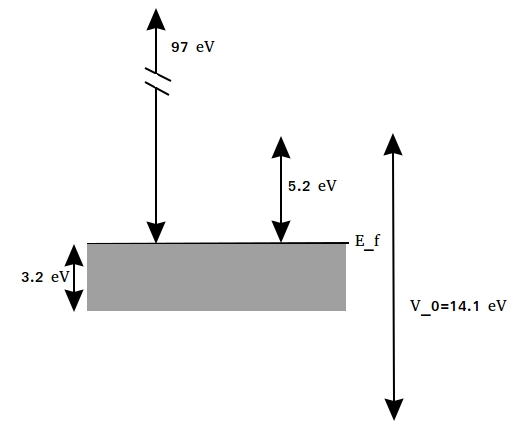
\includegraphics[scale=0.6]{./images/5-8a.jpg}
\label{5-8a}
\end{figure}

\begin{align*}
E_{kin} &= 97 + 14.1 - 5.2 - 3.2\\[3mm]
	&= 102.6\text{ eV}
|k| &= 0.512\sqrt{102.6}\\[3mm]
	&= 5.12\text{ \AA}^{-1}
\end{align*}

with n=1 we have,
\begin{align*}
|g| &= 2* \dfrac{2\pi}{3.61}\\[3mm]
	&= 3.5\text{ \AA}^{-1}
\end{align*}

\[
5.2-3.5 = 1.7\text{ \AA}^{-1} \leftrightarrow |g| = \dfrac{2\pi}{3.61} = 1.7\text{ \AA}^{-1}
\]


\subsection*{b}
\begin{align*}
KE - V_0 &= 102.7\text {eV} - 14.1\text{ eV}\\[3mm]
	&= 88.6\text{ eV}
\end{align*}


\subsection*{c}
for photon \(E=hc/\lambda\)
\begin{align*}
\lambda &= \dfrac{hc}{E}\\[3mm]
	&= \dfrac{1.24\cdot 10^{-6} \text{ eV}\cdot\text{m}}{97\text{ eV}}\\[3mm]
	&= 1.3\cdot 10^{-8}\text{ m}\\[3mm]
	&= 130\text{ \AA}\\[5mm]
k &= \dfrac{2\pi}{130\text{ \AA}}\\[3mm]
	&= 0.048\text{ \AA}^{-1} \ll 1.7\text{ \AA}^{-1}
\end{align*}
so the photon momentum is negligible in comparison to the magnitude of the reciprocal lattice vector.


%%%%%%%%%%%%%%%%%%%%%%%%%%%%%%%%%%%%%%%%%%%%%%%%%%%%%%%%%%%%%%%%%%%%%%%%%%%%%%%%%%%%
%%%%%%%%%%%%%%% PROBLEM 9 %%%%%%%%%%%%%%%%%%%%%
%%%%%%%%%%%%%%%%%%%%%%%%%%%%%%%%%%%%%%%%%%%%%%%%%%%%%%%%%%%%%%%%%%%%%%%%%%%%%%%%%%%%
\newpage
\section*{5.9}





%%%%%%%%%%%%%%%%%%%%%%%%%%%%%%%%%%%%%%%%%%%%%%%%%%%%%%%%%%%%%%%%%%%%%%%%%%%%%%%%%%%%
%%%%%%%%%%%%%%% PROBLEM 10 %%%%%%%%%%%%%%%%%%%%%
%%%%%%%%%%%%%%%%%%%%%%%%%%%%%%%%%%%%%%%%%%%%%%%%%%%%%%%%%%%%%%%%%%%%%%%%%%%%%%%%%%%%
\newpage
\section*{5.10}








\end{document}
